\section{Algorithm verification}
In this section the implementation of Cov-DL and M-SBL are verified separately based on the MSE between the true- and the estimated model parameters.
During the tests on synthetic data sets the segmentation stage is ignored by letting the simulated data form one single segment.    

\subsection{Test of COV-DL}
As seen from the flow diagram figure \ref{fig:flow} COV-DL takes a measurement matrix $\textbf{Y}$, $N$ and $k$ as input and return an estimation $\hat{\textbf{A}}$ of the mixing matrix $\textbf{A}$. The COV-DL algorithm is tested on the two simulations of the deterministic data, specified in section \ref{subseg_simpledata}. 

\subsubsection{COV-DL1}
For $\textbf{Y}$ specified by $N > \widetilde{M}$ and $k\leq \widetilde{M}$, implying COV-DL1, the true and estimated values of $\textbf{A}$ are plotted in figure \ref{fig:cov1_simple} for visual comparison. Note that each matrix is vectorised such that the corresponding entries are compared.  
The resulting $MSE_{A}$ between the true $\textbf{A}$ and the estimated $\hat{\textbf{A}}$ become 
\begin{align*}
MSE_{A} = 1.37
\end{align*}
From figure \ref{fig:cov1_simple} it is seen that the precision of the estimate varies significant for each entry. Though, values within the a similar range are obtained furthermore the $MSE_{A}$ is fairly small suggesting that the estimate is acceptable\todo[inline]{how should we determined this?? and can we give an explanation. \\
jeg har kigget nærmere på dictionary learning funktionen, jeg kan ikke ændre på resultater ved at ændre på k, den er som standard sat til 0.1*n, hvilket er langt mere sparse (under 1 non-zero) end vores system. med ved algorithm ='lars' skulle den godtage k, som ellers for 'omg' bliver overskrevet at standarden. \\
for at undersøge om det igen kan være forholdet mellem A og D, har jeg lavet et system med N=16, M=5, k=4, som skal kunne løsese med dictionary lerning uden brug af covariance domænet. dog bliver resultatet ikke bedre. uanset input så falder A(estimate) altid inden for [-1,1], hvilket er et problem.}  

\subsubsection{COV-DL2}
For $\textbf{Y}$ specified by $N\leq \widetilde{M}$, implying Cov-DL2, the true and estimated values of $\textbf{A}$ are plotted in figure \ref{fig:cov2_simple} for visual comparison. Additionally, is the initial $\textbf{A}$ plotted in the same figure, as standard that is a Gaussian matrix $\textbf{A}_{init}$ which is given to the optimization solver within COV-DL2.    
The resulting $MSE_{A}$ between the true $\textbf{A}$ and the estimated $\hat{\textbf{A}}$ become 
\begin{align*}
MSE_{A} = 2.46 
\end{align*}
From figure \ref{fig:cov2_simple} the estimate $\hat{\textbf{A}}$ shows visual tendencies from the true $\textbf{A}$. However, when it is compared to the initial guess of $\textbf{A}$ it is seen that the resulting estimate have moved further away from the true $\textbf{A}$ compared to $\textbf{A}_{init}$. this suggest some flaw within the optimization process. By printing the convergence message from the used optimization solver it is confirmed that the optimization process was found to be terminated successful. With current function value at $0.0$ after 26 iterations. 
With the resulting cost at 0.0 this suggest that an global minima has been found, but this minima do not correspond to the true $\textbf{A}$.    
To confirm this the following evaluations of the cost function was conducted. 
\begin{align*}
&\text{cost}(\hat{\textbf{A}}) = 0.0\\
&\text{cost}(\textbf{A}_{init}) = 1.564\\
&\text{cost}(\textbf{A}) = 1.809
\end{align*}
These evaluations ensures that the optimization solver have manage to find the solution that minimizes the cost function. By evaluating the cost function with respect to the true $\textbf{A}$ is it seen that it is not a global minimizer to the optimization problem. This suggest that the optimization problem, derived in section \ref{sec:over_det}, do not fulfil the purpose\todo{what word to use here? Jan brugte diverger om noget?}    

\begin{figure}[h]
    \begin{minipage}[t]{.45\textwidth}
		\centering
		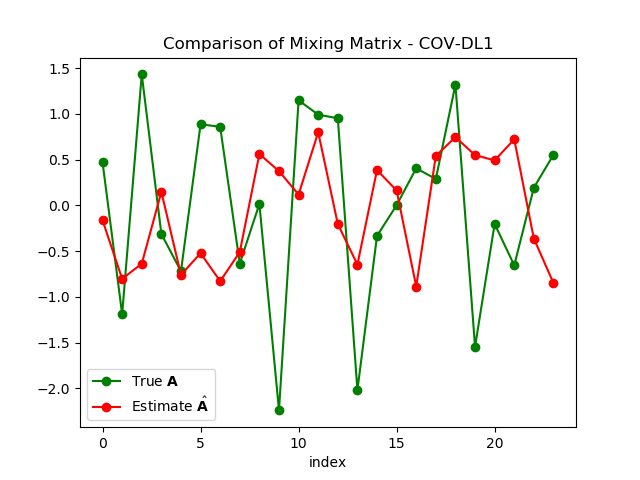
\includegraphics[scale=0.5]{figures/ch_6/COV1_simple.png}
		\caption{Estimated values of $\hat{\textbf{A}}$ compared to the true 				values $\textbf{A}$}
		\label{fig:cov1_simple}
    \end{minipage} 
    \hfill
    \begin{minipage}[t]{.45\textwidth}
        \centering
		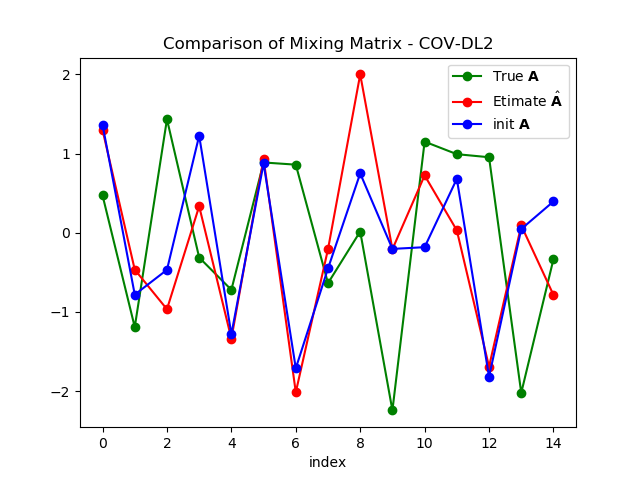
\includegraphics[scale=0.5]{figures/ch_6/COV2_simple.png}
		\caption{The initial $\textbf{A}$ and the estimate $\hat{\textbf{A}}$ 				compared to the true values $\textbf{A}$. }
		\label{fig:cov2_simple}
    \end{minipage}
\end{figure}

\subsubsection{Conclusion to $\hat{\textbf{A}}$}
From the above results is it found that the estimate $\hat{\textbf{A}}$, especially within the COV-DL2 branch, can not be consider a valid estimate of the mixing matrix $\textbf{A}$. It is suggested that the flaw lies within either the  derivation of the optimization problem, more specifically within the assumption made throughout the derivation concerning the relation between $\textbf{A}, \textbf{D}$ and $\textbf{U}$. This statement build upon the success of the(non documented) unit tests of the COV-DL2 algorithm suggesting that the optimisation of D not depending on A is possible(?eller hvad var det vi gjorde?)...
The appearance of this issue may suggest that there is a lack within the published results \cite{Balkan2015}(?tjek)considering the possibility of reconstructing the results.  

Due to the time limitation of the project the error is not investigated further, and it is concluded that the estimate of $\textbf{A}$ is not valid hence it will not be used as an input for the next stage of the algorithm, M-SBL. 

This conclusion suggest that an alternative action must be considered. This is discussed further in section \ref{sec:est_base}

        

\subsection{Alternative to $\hat{\textbf{A}}$}

\subsection{Test of M-SBL}
From the flow diagram figure \ref{fig:flow} it seen that that the M-SBL algorithm takes $\mathbf{A}$ (maybe $k$) and $\mathbf{Y}$ as input. The algorithm is now tested on the same two simple data sets specified by $M = 3$, $k = 4$, $L=1000$ and respectively $N = 5$ and $N = 8$ as used above. 
In order to not let the performance of Cov-DL affect the result of M-SBL it is the true $\mathbf{A}$ which is given as input along with the corresponding $\mathbf{Y}$. The estimate $\hat{\mathbf{X}}$ are plotted in figure \ref{fig:M-SBL_simple1} and \ref{fig:M-SBL_simple2}. Each non-zero signals are now plotted separately for simple visual comparison. Furthermore, note that each compared couple of rows have the same row index, as such the localization of the estimated row can be evaluated.
\begin{figure}[H]
    \begin{minipage}[t]{.45\textwidth}
    	\centering
		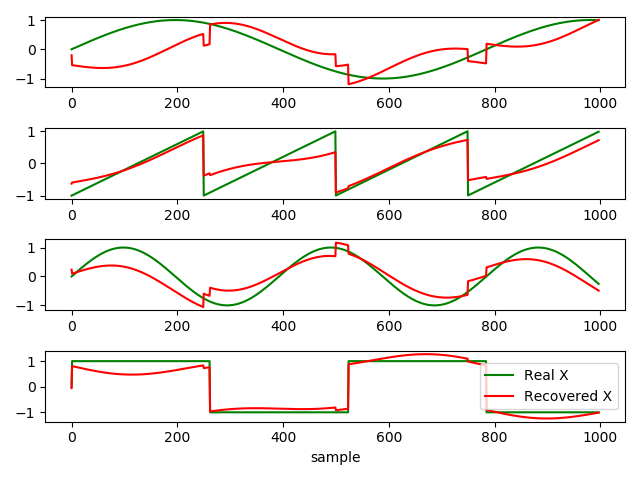
\includegraphics[scale=0.5]{figures/ch_6/M-SBL_simple1.png}
		\caption{Estimated values of $\hat{\textbf{X}}$ compared to the true 					values $\textbf{X}$. From measurement $\textbf{Y}$ specified by $N=5$, $M = 3$, $k=4$ and $L=1000$}
		\label{fig:M-SBL_simple1}
    \end{minipage} 
    \hfill
    \begin{minipage}[t]{.45\textwidth}
        \centering
		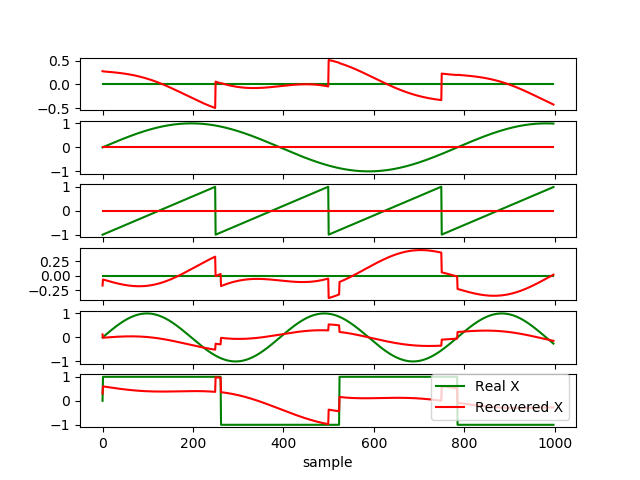
\includegraphics[scale=0.5]{figures/ch_6/M-SBL_simple2.png}
		\caption{Estimated values of $\hat{\textbf{X}}$ compared to the true 				values $\textbf{X}$. From measurement $\textbf{Y}$ specified by $N=8$, $M = 3$, $k=4$ and $L=1000$ }
		\label{fig:M-SBL_simple2}
    \end{minipage}
\end{figure}
The resulting MSE between the true $\textbf{X}$ and the estimated $\hat{\textbf{X}}$ from figure \ref{fig:M-SBL_simple1} where $N = 5$, averaged over every row, become 
\begin{align*}
X_{MSE} = 0.131 
\end{align*}
From figure \ref{fig:M-SBL_simple1} it is seen that all four source signals are recovered at the right location. As suggested by the achieved MSE it the estimates are not exact, but it is clear that the estimates manage to follow the right pattern at the right location. By this plot an error margin are established(?).  

The resulting MSE between the true $\textbf{X}$ and the estimated $\hat{\textbf{X}}$ from figure \ref{fig:M-SBL_simple2} where $N = 8$ thus more sparse, become 
\begin{align*}
X_{MSE} = 0.145 
\end{align*}
From figure \ref{fig:M-SBL_simple2} it is seen that first source signal are recovered at the third entry, that is one dislocation, while the rest are recovered at the right location. This indicate that the algorithm can manage to locate the source signal however the more options the more greater chance of dislocation.     

\subsubsection*{Possibilities of $N=k$}
\begin{itemize}
	\item The true $N$ is unknown for real EEG measurements, as it change for every brain
	\item Therefore, we do not know the amount of activation inside the brain, but it is those which are of interest in this thesis.
	\item Due to the method for determine the mixing matrix $\textbf{A}$ the ration between $N$ and $k$ do not affect the result, hence there are no argument against letting $N=k$ which will lower the computational complexity.\todo[inline]{do the same argument regarding $N=k$ hold for the determination of $\textbf{X}$? after the awareness that we do not need to provide $k$ to M-SBL as it has been done so far.}    
\end{itemize}

\section{Test on AR data and model fitting}
The implemented algorithms are now tested on the simulated autoregressive data sets which resembles the real EEG measurements. Furthermore it is sought to improve the model by fitting specific model variables to the data. In this case it is the Cov-DL algorithm which can be adjusted for the overdetermined case where Cov-DL2 is used.      

\subsection{Model Fitting}
Two model variables are now considered with the purpose of improving the performance of the COV-DL algorithm. The initial A given to the optimization problem \eqref{eq:Cov_DL2} within COV-DL2, and the segmentation size used within the covariance domain.   
\subsubsection*{Initial $\textbf{A}$}
Consider the COV-DL algorithm in the case where the system transformed into the covariance domain results in an overdetermined system. In this case the COV-DL2 branch of the algorithm is used. 
When estimating the mixing matrix $\mathbf{A}$ a matrix $\mathbf{D}$ is used in the process. For the over-determined system \ref{sec:over_det} $\mathbf{D}$ is found by solving the optimisation problem \eqref{eq:Cov_DL2} with respect to $\hat{\textbf{A}}$. To solve the optimization problem an initial $\mathbf{A}_{\text{ini}}$ is given. The choice of this initial $\mathbf{A}_{\text{ini}}$ may affect how the good an estimate the recovered mixing matrix $\mathbf{A}$ is.
Three different choices of $\mathbf{A}_{\text{ini}}$ are considered:
\begin{itemize}
\item[-] A matrix $\mathbf{A1}$ drawn from a continuous uniform distribution in the half-open interval $[0.0, 1.0)$
\item[-] A matrix $\mathbf{A2}$ drawn from a uniform distribution in the half-open interval $[-1.0, 1.0)$
\item[-] A matrix $\mathbf{A3}$ drawn from a Gaussian distribution with mean 0 and variance 1
\end{itemize}
The test of different initial $\mathbf{A}_{\text{ini}}$ is performed on the 
an AR data set specified by $N=5$ $M = 3$, $k = 4$ and $L = 1000$. 
The MSE of the three tests are seen in table \ref{tab:iniA} 
\begin{table}[H]
\centering
\begin{tabular}{|l|l|l|l|} 
\hline
                          & \textbf{A1} & \textbf{A2} & \textbf{A3} \\
\hline $\text{MSE}_{\mathbf{A}}$ &   2.15          & 2.00            & 1.88\\
\hline           
\end{tabular}
\caption{Resulting MSE for varying initial A, used within COV-DL2.}
\label{tab:iniA}
\end{table}
\todo[inline]{is it okay that we do not include the mse of X here, I don't think is any reasoning to do it, but it should be check later whether the error of A follows the error of X as it is asumped at this moment.}
From the results it is seen that \textbf{A3} achieves the lowest MSE, thus an Gaussian distributed initial $\textbf{A}$ will be used.    
 
% old results
%For the test we are looking at a system of size $M = 8$, $k = 16$ and $L = 1000$. Furthermore, for the Cov-DL the data has been divided in segments of 10 samples leading to 100 segments.
%\begin{figure}[H]
%\centering
%    \begin{minipage}[t]{.45\textwidth}
%        \centering
%		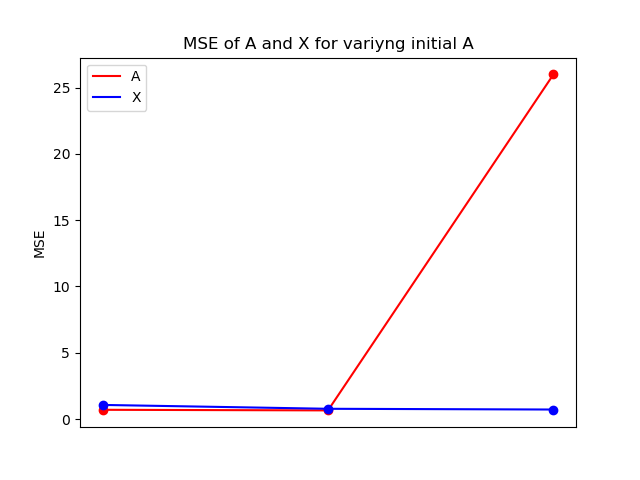
\includegraphics[scale=0.5]{figures/chapter6/Mix_Error_initial_A_m8_k16_L1000.png}
%		\subcaption{Simple Data Set - Estimated A}
%    \end{minipage} 
%    \hfill
%    \begin{minipage}[t]{.45\textwidth}
%        \centering
%		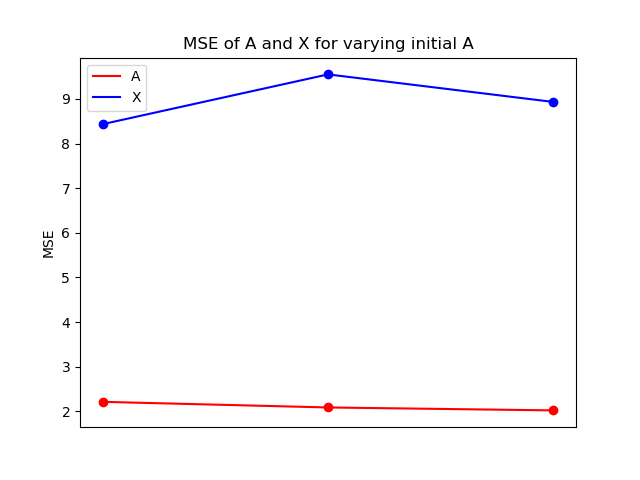
\includegraphics[scale=0.5]{figures/chapter6/AR_Error_initial_A_m8_k16_L1000.png}
%		\subcaption{Autoregressive Data Set - Estimated A}
%    \end{minipage}
%    \begin{minipage}[t]{.45\textwidth}
%        \centering
%		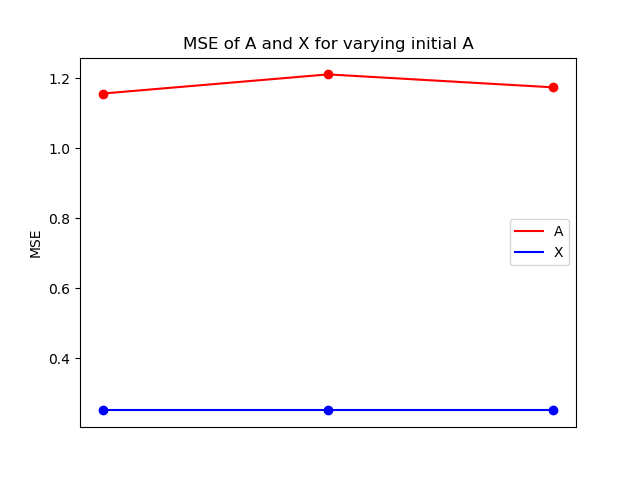
\includegraphics[scale=0.5]{figures/chapter6/Mix_Error_initial_A_m8_k16_L1000_RealA.png}
%		\subcaption{Simple Data Set - Real A}
%    \end{minipage} 
%    \hfill
%    \begin{minipage}[t]{.45\textwidth}
%        \centering
%		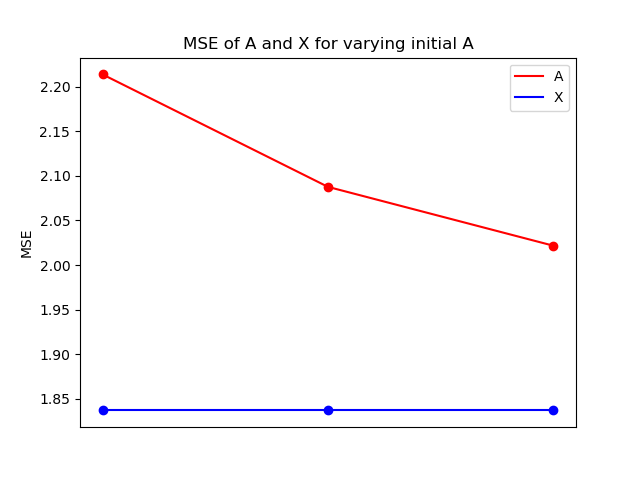
\includegraphics[scale=0.5]{figures/chapter6/AR_Error_initial_A_m8_k16_L1000_RealA.png}
%		\subcaption{Autoregressive Data Set - Real A}
%    \end{minipage}
%\caption{}
%\label{fig:initialA}
%\end{figure}
%\noindent
%The MSE values of each tests -- estimated and real mixing matrix $\mathbf{A}$ -- can be seen in table \ref{tab:iniA}. For the real mixing matrix the MSE values of source matrix $\mathbf{X}$ are identical because the real mixing matrix is not influenced by the three different initial $\mathbf{A}_{\text{ini}}$.
%\begin{table}[H]
%\begin{minipage}{.5\linewidth}
%\centering
%\begin{tabular}{|c|c|c|c|}
%\hline 
% & $\mathbf{A1}$ & $\mathbf{A2}$ & $\mathbf{A3}$ \\ 
%\hline 
%MSE of $\mathbf{A}$ & 1.16 & 1.21 & 1.17 \\ 
%\hline 
%MSE of $\mathbf{X}$ & 0.69 & 0.66 & 0.81 \\ 
%\hline 
%\end{tabular} 
%\subcaption{Simple Data Set - estimated $\mathbf{A}$}
%\end{minipage}
%\begin{minipage}{.5\linewidth}
%\centering
%\begin{tabular}{|c|c|c|c|}
%\hline
% & $\mathbf{A1}$ & $\mathbf{A2}$ & $\mathbf{A3}$ \\ 
%\hline 
%MSE of $\mathbf{A}$ & 2.21 & 2.09 & 2.02 \\ 
%\hline 
%MSE of $\mathbf{X}$ & 8.43 & 9.55 & 8.93 \\ 
%\hline
%\end{tabular} 
%\subcaption{Autoregressive Data Set - estimated $\mathbf{A}$}
%\end{minipage}
%\begin{minipage}{.5\linewidth}
%\centering
%\begin{tabular}{|c|c|c|c|}
%\hline 
% & $\mathbf{A1}$ & $\mathbf{A2}$ & $\mathbf{A3}$ \\ 
%\hline 
%MSE of $\mathbf{A}$ & $\times$ & $\times$ & $\times$ \\ 
%\hline 
%MSE of $\mathbf{X}$ & 0.25 & 0.25 & 0.25 \\ 
%\hline 
%\end{tabular} 
%\subcaption{Simple Data Set - real $\mathbf{A}$}
%\end{minipage}
%\begin{minipage}{.5\linewidth}
%\centering
%\begin{tabular}{|c|c|c|c|}
%\hline
% & $\mathbf{A1}$ & $\mathbf{A2}$ & $\mathbf{A3}$ \\ 
%\hline 
%MSE of $\mathbf{A}$ & $\times$ & $\times$ & $\times$ \\ 
%\hline 
%MSE of $\mathbf{X}$ & 1.84 & 1.84 & 1.84 \\ 
%\hline
%\end{tabular} 
%\subcaption{Autoregressive Data Set - real $\mathbf{A}$}
%\end{minipage}
%\caption{(a) This are the MSE values achieve from the simple data set and (b) is the MSE values achieved from the autoregressive data set.}
%\label{tab:iniA}
%\end{table}
%\noindent
%From \ref{tab:iniA} we see that the MSE values for our estimated mixing matrix $\mathbf{A}$ are overall small compared to both data sets. However, if we look at the results for the source matrix there are a big different from the simple data set and the autoregressive data set and comparing it to the results with the real mixing matrix. 
%As the autoregressive data set have a higher amplitude in the data than the simple data set, the error will become larger. 
%
%If we look at the initial $\mathbf{A}_{\text{ini}}$ drawn from the Gaussian distribution we have a small error for the mixing matrix in the autoregressive data set while the error from the simple data set also is low. The error for source matrix is the highest value for the simple data set but comes second in the autoregressive data set. As we want to take into account that the autoregressive data set resemble the EEG measurement most we conclude that the initial $\mathbf{A}_{\text{ini}}$ from the Gaussian distribution would be the best choice in Cov-DL.

\subsubsection{Segmentation in Covariance domain}
For the Cov-DL algorithm when estimating the mixing matrix $\mathbf{A}$ the measurement matrix is transformed into the covariance domain as part of the recovering process. During the transformation the measurement matrix $\mathbf{Y}$ is divided into segments consisting of $L_s$ samples each.
During this test different numbers of samples within a segment will be tested to see how this affect the performance of the algorithm.

The autoregressive data sets,  $M = 3$, $k = 4$ and $L = 1000$ samples and with respectively $N = 5$ and $N=8$, will be used for the testing. With $k = 4$ the number of segments can not be less than the number of sources. For this system each segment can have maximum $L_s = 200$ corresponding to minimum 5 segments. 

For the test, six different number of samples within each segments will be tested, $L_s = \{ 10, 20, 30, 50, 100, 150, 200 \}$. Furthermore, each $L_s$ will be run 10 times and the output of the test will be average such that each $L_s$ have one average MSE.
%\begin{figure}[H]
%\centering
%    \begin{minipage}[t]{.45\textwidth}
%        \centering
%		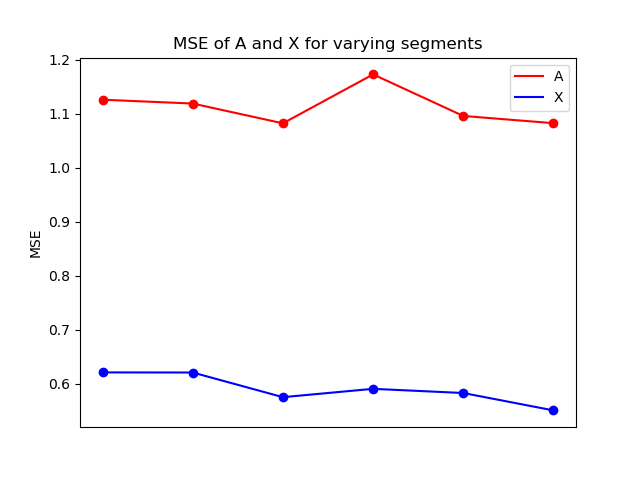
\includegraphics[scale=0.5]{figures/chapter6/Mix_Error_vary_covseg_m8_k16_L1000}
%		\subcaption{Simple Data Set - Estimated A}
%    \end{minipage} 
%    \hfill
%    \begin{minipage}[t]{.45\textwidth}
%        \centering
%		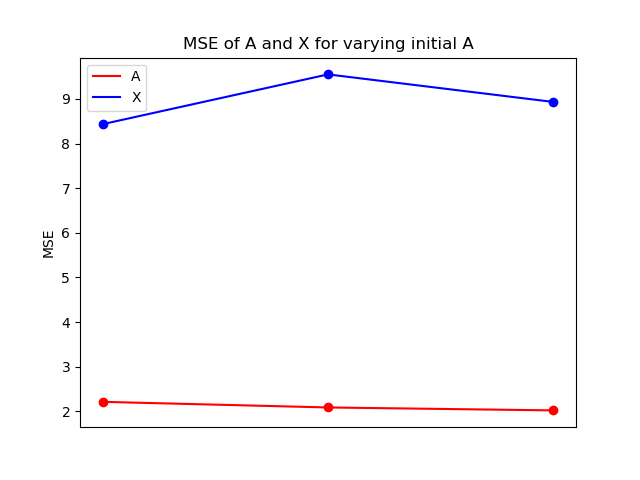
\includegraphics[scale=0.5]{figures/chapter6/AR_Error_initial_A_m8_k16_L1000.png}
%		\subcaption{Autoregressive Data Set - Estimated A}
%    \end{minipage}
%    \begin{minipage}[t]{.45\textwidth}
%        \centering
%		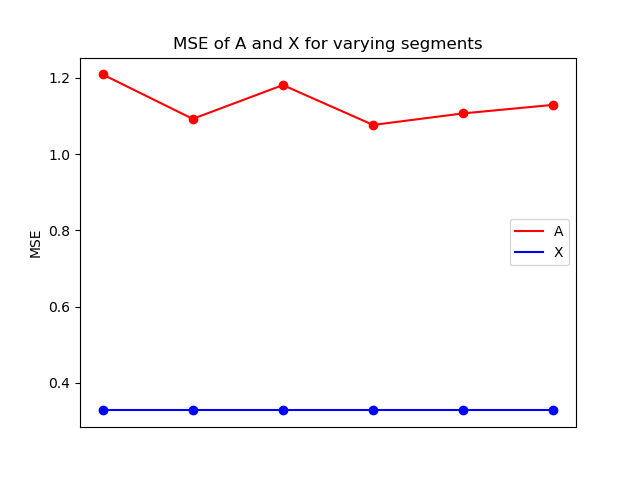
\includegraphics[scale=0.5]{figures/chapter6/Mix_Error_vary_covseg_m8_k16_L1000_RealA.png}
%		\subcaption{Simple Data Set - Real A}
%    \end{minipage} 
%    \hfill
%    \begin{minipage}[t]{.45\textwidth}
%        \centering
%		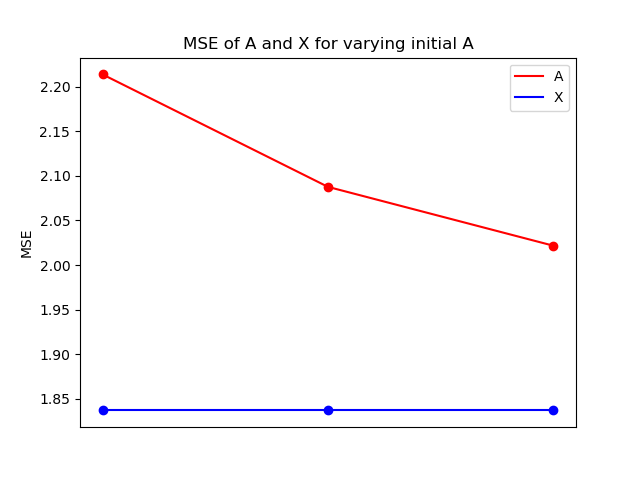
\includegraphics[scale=0.5]{figures/chapter6/AR_Error_initial_A_m8_k16_L1000_RealA.png}
%		\subcaption{Autoregressive Data Set - Real A}
%    \end{minipage}
%\caption{}
%\label{fig:seg}
%\end{figure}
%\noindent
%The MSE values of each tests -- estimated and real mixing matrix $\mathbf{A}$ -- can be seen in table \ref{tab:seg}\todo[inline]{hvordan kan det være der kun er 3 punkter for AR dataen?\\
%\textbf{X} fejlen er mærkelig høj her, er der en grund til det}.

\begin{table}[H]
\centering
\begin{minipage}{.45\textwidth}
\centering
\begin{tabular}{|c|c|c|c|c|c|c|c|}
\hline 
& 10 & 20 & 30 & 50 & 100 & 150 & 200 \\ 
\hline 
Average MSE of $\hat{\mathbf{A}}$ & 1.86 & 2.14 & 2.21 & 2.03 & 2.31 & 1.89 & 2.06 \\ 
\hline
\end{tabular} 
\caption{MSE values from measurement specified by $N=5$, $M = 3$, $k = 4$ and $L = 1000$ achieved from the used of Cov-DL2}
\label{tab:seg1}
\end{minipage}
\\
\begin{minipage}{.45\textwidth}
\centering
\begin{tabular}{|c|c|c|c|c|c|c|c|}
\hline 
& 10 & 20 & 30 & 50 & 100 & 150 & 200 \\ 
\hline 
Average MSE of $\hat{\mathbf{A}}$ & 1.29 & 1.37 & 1.22 & 1.16 & 1.46 & 1.20 & 1.32 \\ 
\hline
\end{tabular} 
\caption{MSE values from measurement specified by $N=8$, $M = 3$, $k = 4$ and $L = 1000$ achieved the used of Cov-DL1.}
\label{tab:seg2}
\end{minipage}
\end{table}
\noindent
Overall, in table \ref{tab:seg1} and \ref{tab:seg2} there is not a big variation between the MSE values of both data sets. One could argument that the number of samples within each segment does not affect the performance of the algorithms as much and therefore is more free choice.

\subsection{Test on AR data}
Both algorithms are now test on AR data set ..... missing description


\begin{figure}[H]
    \begin{minipage}[t]{.45\textwidth}
    	\centering
		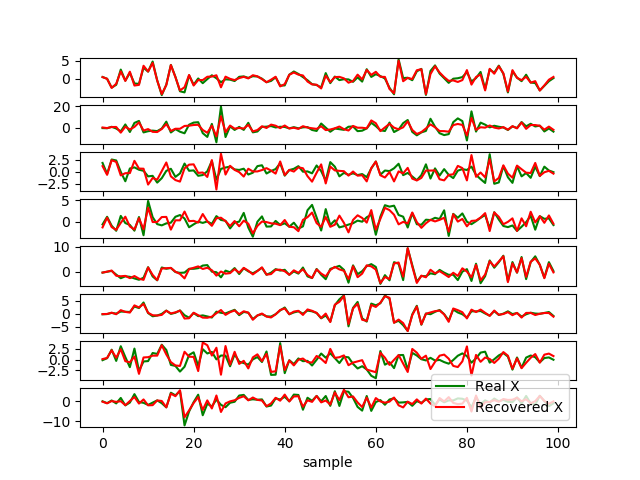
\includegraphics[scale=0.5]{figures/ch_6/M-SBL_AR1.png}
		\caption{ $N=5$, $M = 3$, $k=4$ and $L=1000$  - True $\textbf{A}$}
		\label{fig:AR1}
    \end{minipage} 
    \hfill
    \begin{minipage}[t]{.45\textwidth}
        \centering
		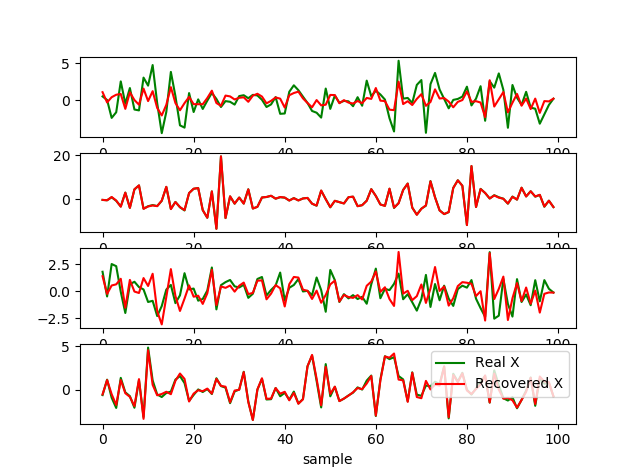
\includegraphics[scale=0.5]{figures/ch_6/M-SBL_AR2.png}
		\caption{$N=k=4$ $M = 3$ and $L=1000$ - True $\textbf{A}$}
		\label{fig:AR2}
    \end{minipage}
\end{figure}


MSE for $N=5$, $k=4$ is 2.17\\
MSE for $N=k=4$ is 0.682\\


 
